\documentclass[a4paper]{article}

\usepackage[T1]{fontenc}
\usepackage{textcomp}
\usepackage{xcolor}
\usepackage{url}
\usepackage{stackengine}
\usepackage [english]{babel}
\usepackage [autostyle, english = american]{csquotes}
\usepackage{courier}
\usepackage{listings}
\usepackage{minted}
\usepackage{graphicx}
\usepackage{lmodern}
\usepackage{mathtools}
\usepackage{amsfonts}
\usepackage{float}



\lstset{
  basicstyle=\footnotesize\ttfamily,
  frame=single,
  numbers=left,
  captionpos=b
}


\begin{document}


\title{AI Assessed Exercise}

\author{Ross Meikleham 1107023m}

\maketitle


\section{Chapter 1 - Design}


\textbf{PEAS}
\begin{itemize}
\item \textbf{Performance} 
\item \textbf{Environment} 
\item \textbf{Sensors} 
\item \textbf{Actuators} 
\end{itemize}


\section{Chapter 2 - Theory}


\subsection{Extracting Short Term Signals} \label{sec:extract}

The properties of a signal are stable in the short-term but change, so we need
to use a sliding window that spans the entire signal at regular intervals of time.
In this exercise we use a rectangular window. The samples inside a rectangular window
have the value 1, and samples outside the window have the value 0.

A rectangular window is defined as follows: 

\begin{equation}
w[n] =
    \begin{cases}
        1, & 0 \leq n \leq N-1\\
        0, & \text{otherwise}
    \end{cases}
\end{equation}


\subsubsection{Extracting Energy} \label{sec:energy}

The equation for calcuating the energy is as follows:
\begin{equation}
 E[n] = \sum_{k=-\infty}^{\infty}\frac{(s[k])^2}{N}.w[n-k]
\end{equation}

However, since we're using a rectangular window; we know that $w[n]$ is 0 for k values in which $n - k$
is outside of the window, and as a result the equation at these k values will always result in 0. 
So we can restrict the sum over the values in which $n - k$ is inside the window.

From this we can extract the energy with the rectangular window using the following
equation:

\begin{equation}
 E[n] = \sum_{k=n-N+1}^{n}\frac{(s[k])^2}{N}.w[n-k]
\end{equation}


Implementing this and calculating the window size



\subsubsection{Extracting Magnitude}

The equation for calculating the magnitude is as follows:

\begin{equation}
 E[n] = \sum_{k=-\infty}^{\infty}\frac{|s[k]|}{N}.w[n-k]
\end{equation}

Using the same reasoning as in section \ref{sec:energy} we can extract the
magnitude with the rectangular window using the following equation:

\begin{equation}
 E[n] = \sum_{k=n-N+1}^{n}\frac{|s[k]|}{N}.w[n-k]
\end{equation}



\subsubsection{Extracting Zero Crossing Rate}

The Zero Crossing Rate provides the rate at which a signal changes from
positive to negative, or vice-versa.

The equation for calculating the Zero-Crossing Rate(ZCR) is as follows:

\begin{equation}
 E[n] = \frac{1}{2N}\sum_{k=-\infty}^{\infty}|sign(s[k] - sign(s[k-1]])|.w[n-k]
\end{equation}

where
\begin{equation}
sign[n] =
    \begin{cases}
        -1, & n  < 0\\
         1, & n  > 0\\
         0, & n  = 0
    \end{cases}
\end{equation}

Using the same reasoning as in section \ref{sec:energy} we can extract the
ZCR with the rectangular window using the following equation:

\begin{equation}
 E[n] = \frac{1}{2N}\sum_{k=n-K+1}^{N}|sign(s[k] - sign(s[k-1]])|.w[n-k]
\end{equation}


\subsection{Decisions}

The exercise is a binary classification problem in that we need to determine
if a given sample contains speech or not. The classification property is the 
presence of speech.

$R(B_i,\vec x)$ is called Bayes Risk, where in this case 

\begin{equation}
R(B_1|\vec x) = \pi(B_1|C_1)p(C_1|\vec x) + \pi(B_1|C_2)p(C_2|\vec x) 
\end{equation}

\begin{equation}
R(B_2|\vec x) = \pi(B_2|C_1)p(C_1|\vec x) + \pi(B_2|C_2)p(C_2|\vec x) 
\end{equation}

where $B_i$ is the correct action for decision $C_i$.
$\vec x$ is a set of features.


We can manipulate the Risk equations above to get the following:

\begin{equation}
\frac{p(\vec x|C_1)}{p(\vec x|C_2)} > \frac{\pi(B_1|C_2) - \pi(B_2|C_2)}{\pi(B_2|C_1) - \pi(B_1|C_1)}.\frac{p(C_2)}{p(C_1)} 
\end{equation}

If the likelihood ratio is larger than the expression on the right hand side, the decision made is $B_1$ otherwise
the decision made is $B_2$

We need to be able to calculate a value for the amount of loss calculated
from the prediction value compared to the actual value.

For this exercise we use a Zero-One Loss function to calculate the loss, which is defined as follows:

\begin{equation}
\pi(B_i|C_i) =  
    \begin{cases}
        0, & i == j \\
        1, & i \neq j
     \end{cases}
\end{equation}



\subsection{Feature Values}

We have three feature values for each sample which we use to predict which class a sample belongs to.
\begin{itemize}
\item The logarithm of the average value of the short-term energy signal
\item The logarithm of the average value of the short-term magnitude signal
\item The average value of the Zero Crossing Rate signal
\end{itemize}

These values can be computed after using the methods described in section \ref{sec:extract}
to extract the ZCRs, short-term energy signals, and the short-term magnitude signals.

With the given set of 100 samples we then compute the feature values for each sample
and then plot them against each other; resulting in the following graphs:

\begin{figure}[H]
\begin{center}
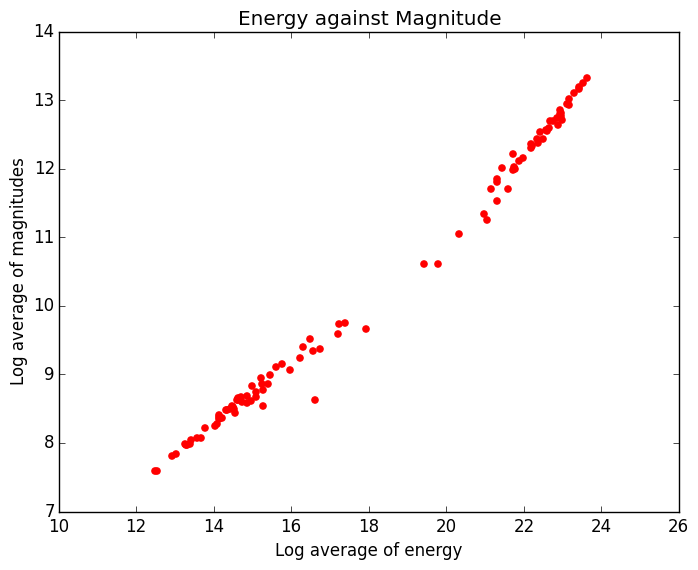
\includegraphics[width=\textwidth, height=\textheight, keepaspectratio]{../src/AI/Lab2/eam.png}
\caption{.}
\label{plot1}
\end{center}
\end{figure}


\begin{figure}[H]
\begin{center}
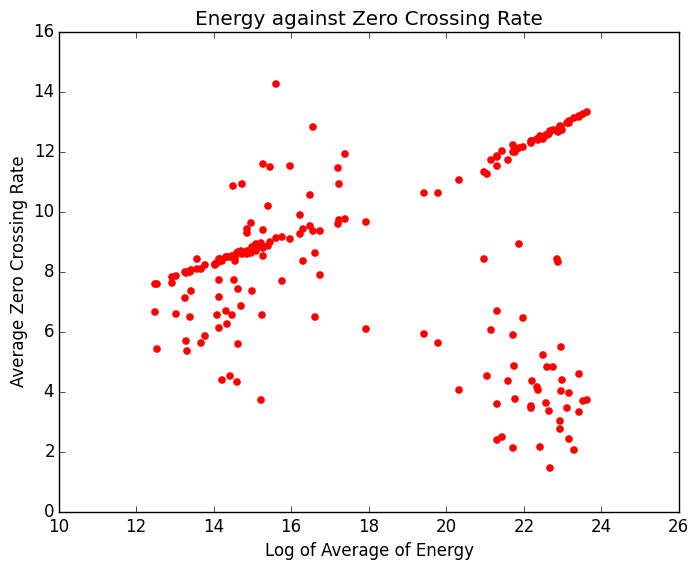
\includegraphics[width=\textwidth, height=\textheight, keepaspectratio]{../src/AI/Lab2/eac.png}
\caption{.}
\label{plot2}
\end{center}
\end{figure}


\begin{figure}[H]
\begin{center}
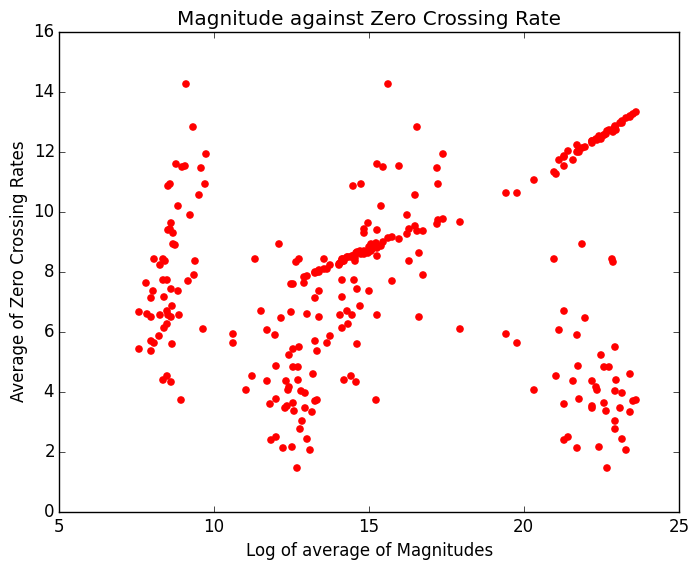
\includegraphics[width=\textwidth, height=\textheight, keepaspectratio]{../src/AI/Lab2/maz.png}
\caption{.}
\label{plot3}
\end{center}
\end{figure}


\subsection{Gaussian Discriminant} \label{sec:gauss}

The following is a set of discriminant functions:
\begin{equation}
G = \lbrace \gamma_1(\vec x),...,\gamma_L(\vec x) \rbrace
\end{equation}

We select the largest $\gamma_k(\vec x)$ in G, the decision made is
then $C_k$. 

For our case using a Zero-One loss function we obtain the following discriminant functions:

\begin{equation}
\log(\gamma_i(\vec x)) \simeq \log(p(\vec x|C_i)) + \log(p(C_i))
\end{equation}

The Univariate Gaussian is a probability density function

\begin{equation}
p(x) = \frac{1}{\sqrt{2 \pi \sigma}}e^{-\frac{(x - \mu)^2}{2 \sigma^2}}
\end{equation} 

Where $\mu$ is the mean, and $\sigma^2$ is the variance.

We assume that the distribution of each of our features is a
guassian distribution.

We then get the following Gaussian discriminant functions:

\begin{equation}
\log(\gamma_i(\vec x)) = -\log\sqrt{2 \pi \sigma} - \frac{(x - \mu_i)^2}{2 \sigma^2_i} + \log(p(C_i))
\end{equation}

There is one problem with using a univariate gaussian discriminant in this case as we have 3 seperate
feature variables, and a univariate gaussian only operates on a single variable. We need to modify
our discriminant functions to work with this.


\begin{equation}
M_i = \lbrace \alpha_{1_i}(\vec x_i),...,\alpha_{L_i}(\vec x_i) \rbrace
\end{equation}

\begin{equation}
\begin{split}
\log(\gamma_k(\vec x))) &= \log(\alpha_{k_1}(\vec x)) + \log(\alpha_{k_2}(\vec x)) + \log(\alpha_{k_3}(\vec x))\\
 &= \log(\alpha_{k_1}(\vec x)) \alpha_{k_2}(\vec x) \alpha_{k_3}(\vec x))
\end{split}
\end{equation}


Where $M_i$ is a set of univariate gaussian distribution functions on the ith feature,
for $ 1 \leq i \leq 3$.

From this we can generate gaussian discriminant functions from a subset of our data to
predict whether a sample has speech in it or not.


\section{Chapter 3 - Experiments}

From our samples we extract the features using a window size of 15ms, then we randomly
split the data into 10 disjoint subsets, ensuring that each subset contains equal amounts
of voice samples and silence samples. 

We then take one of the subsets as a test set and then 
concatonate the reminaing subsets into a single training set (using 90\% of the data
as test data, and 10\% as training data). We generate our gaussian discriminant functions
on the training data using the method described in section \ref{sec:gauss}. We then
use the gaussian discriminant functions to predict which class each sample in the training
set belongs to and compute the loss using our loss function. We then average the total
loss.

We then take another subset as the training set and perform the same steps, and add the average loss
to the previous average loss.

We repeat this until all subsets have been used as the training set, and divide the total average
loss over the amount of subset to obtain the average.

With this I averaged a loss of 0.05. Which corresponds to 5\%. So the cross validation
approach was around 95\% accurate.



\newpage

\appendix

\section{Lab1 Processing Code} (Haskell)

\subsection{Lab1.hs}
\inputminted{haskell}{../src/AI/Lab1/Lab1.hs}

\subsection{Main.hs}
\inputminted{haskell}{../src/AI/Lab1/Main.hs}

\section{Lab1 Plotting Code} (Python)
\inputminted{python}{../src/AI/Lab1/plotting.py}


\section{Lab2 Processing Code (Haskell)}

\subsection{Lab2.hs}
\inputminted{haskell}{../src/AI/Lab2/Lab2.hs}

\subsection{Main.hs}
\inputminted{haskell}{../src/AI/Lab2/Main.hs}


\section{Lab2 Plotting Code (Python)}
\inputminted{python}{../src/AI/Lab2/plotting.py}



\end{document}
